\section{ESP Aufbau}
\label{sec:ESP Aufbau}

\noindent Encapsulating Security Payload (ESP) wird bei \ac{IPsec} (VPN) eingesetzt. Es gewährleistet die Vertraulichkeit und Integrität von Paketen und kümmert sich um die Authentisierung. Durch diese Integritätssicherung werden Pakete vor Manipulation geschützt. ESP verschlüsselt, im Unterschied zu Authentication Header (AH), die Nutzdaten. Bei AH werden nur die Integrität und Echtheit sichergestellt.\cite{elektronik_kompendium}

\noindent Der ESP Header wird zwischen dem IP Header und dem darunterliegenden Protokoll eingefügt (Transport Mode), oder es kapselt das ganze IP-Paket (Tunnel Mode).\cite{rfc4303}

\noindent Der Tunnel Mode wird vor allem bei der Verbindung zwischen zwei Netzwerken über eine unsichere Verbindung eingesetzt. Der Modus unterstützt aber prinzipiell alle Arten von VPN-Anwendungen. Bei dieser Verwendung wird das ganze IP-Paket verschlüsselt und in ein neues IP-Paket verpackt. So wird das gesamte Paket durch ESP abgeschirmt und die eigentliche IP-Adresse des Absenders ist nicht mehr ersichtlich. Diese Methode hat natürlich einen gewissen Overhead. Es kommen 8 Byte für den ESP-Header, 16-20 Byte ESP-Trailer und für den neuen IP-Header 20 Byte hinzu.\cite{elektronik_kompendium}

\begin{figure}[H]
    \begin{center}
        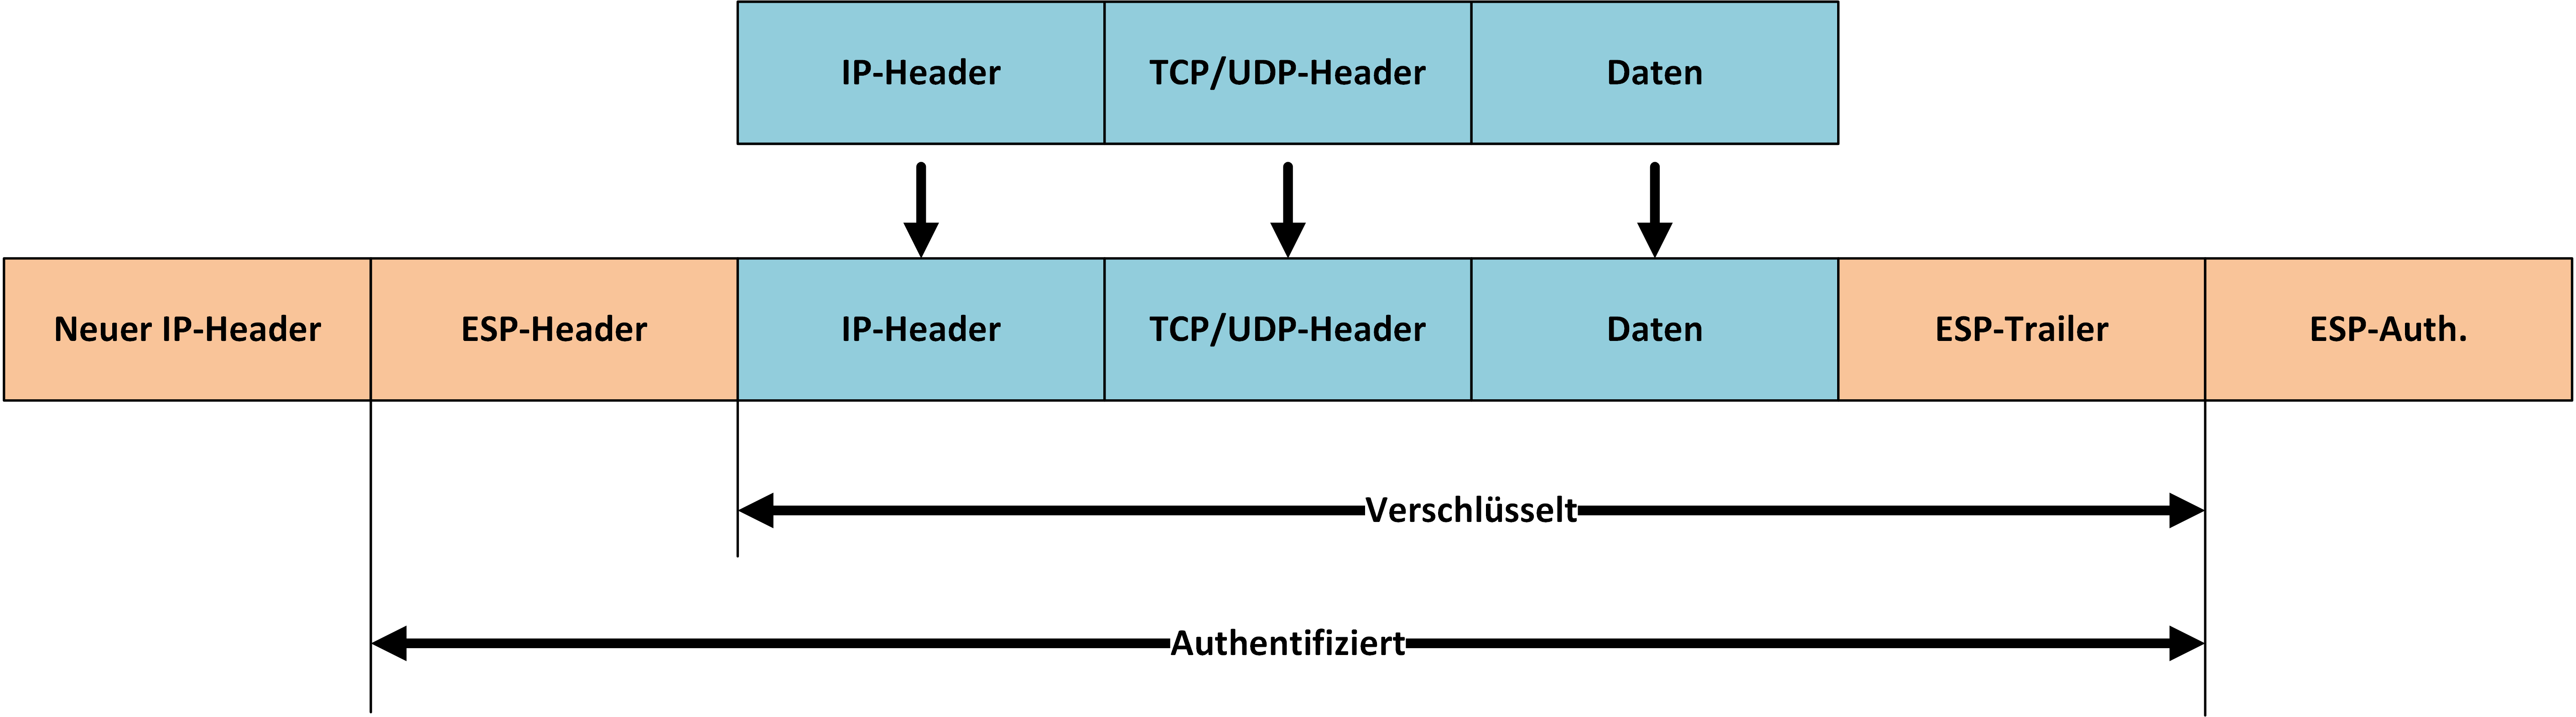
\includegraphics[trim=1 0 0 0,clip,width=\textwidth]{mainpart/analyse/img/ESP_Tunnelmode.png}
    \end{center}
    \caption{Aufbau eines Pakets im Tunnelmode}
\end{figure}

\noindent Bei einer Situation, in der nur zwei Rechner miteinander verbunden werden, kann der Transportmodus verwendet werden. Dieser Modus unterstützt nur Host-to-Host Verbindungen. Da es für \ac{IPsec} nicht unbedingt notwendig ist IP-Pakete vollständig neu zu entkapseln, können beim Transport Mode der originale IP-Header verwendet werden. Es kommen 8 Byte ESP-Header und 16-20Byte ESP-Trailer hinzu. Damit wird der Overhead kleiner, da man keinen zusätzlichen IP-Header benötigt.\cite{elektronik_kompendium}

\begin{figure}[H]
    \begin{center}
        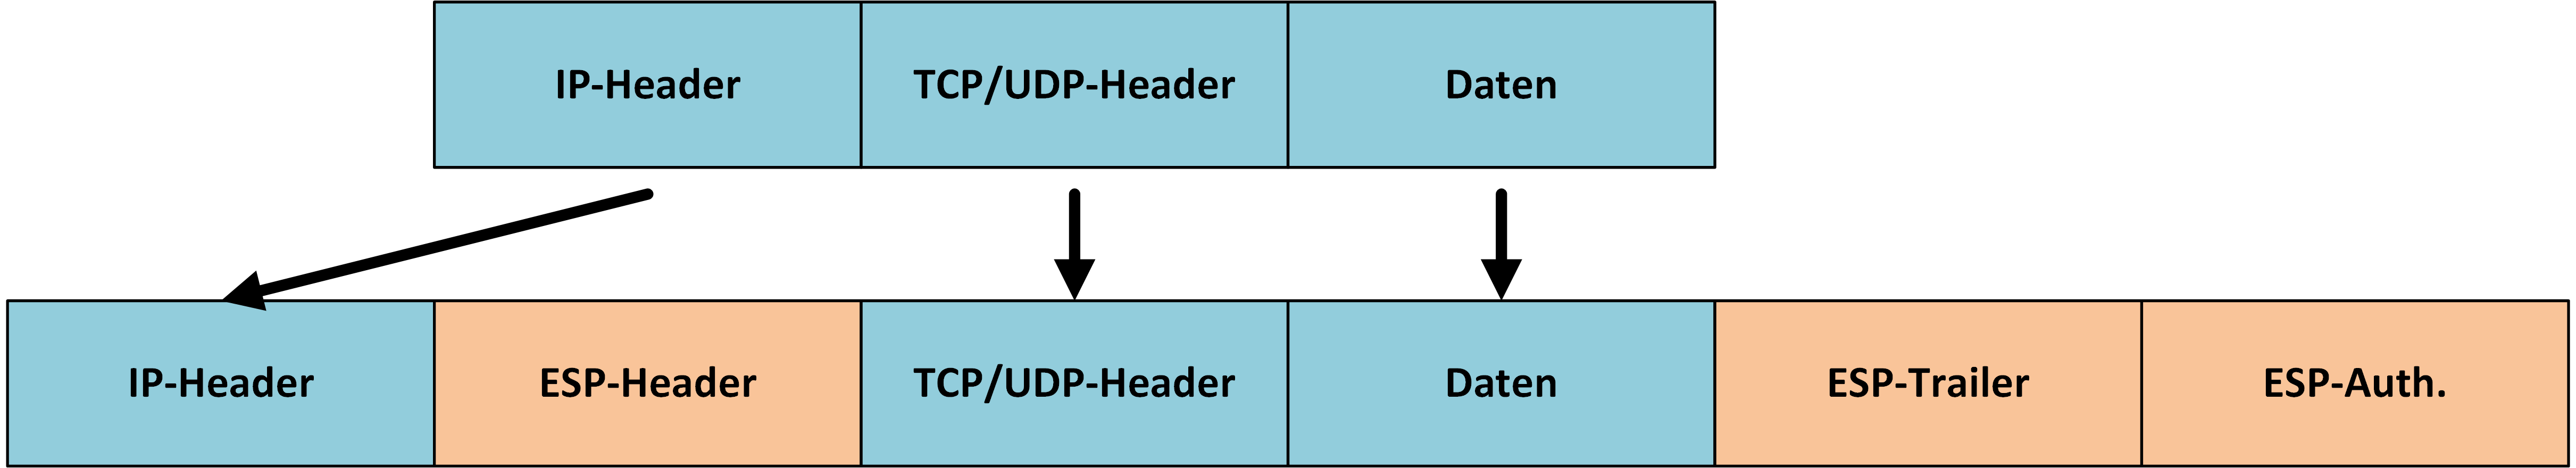
\includegraphics[trim=1 0 0 0,clip,width=\textwidth]{mainpart/analyse/img/ESP_Transportmode.png}
    \end{center}
    \caption{Aufbau eines Pakets im Transportmode}
    %\label{fig:AST_function_call_with_and_without_template_id}
\end{figure}


\textbf{Wichtige Felder}

\begin{table}[H]
\begin{tabularx}{\textwidth}{l|>{\raggedright\arraybackslash}X} 
\hline
Security Parameters\\ Index (SPI) 32bits & Dieser zufällig festgelegte Wert in Kombination mit der IP-Adresse des Ziels wird für eine Identifikation der Verbindung benötigt. Bei jeder neuen Verbindung wird die SPI neu gesetzt.                                                                                                                                                                                                                                                                         \\ \hline
Sequence Number 32bits & Die Sequence Number wird für jedes Paket gesetzt und wird danach für jedes neue Paket um 1 erhöht. Bei einer neuen Verbindung wird die Sequence Number stets auf 1 gesetzt. Falls Anti-Replay eingesetzt wird (standardmässig aktiviert) darf sich die Sequence Number nicht wiederholen. Daher wird, bevor das 2\^{}32 Paket gesendet wird, die Verbindung zurückgesetzt und eine neue SPI ausgehandelt. Damit ist auch die Sequence Number wieder zurückgesetzt. \\
\hline
\end{tabularx}
\caption{Wichtige ESP Felder}
\end{table}